%% V1.0
%% by Gabriel Garcia, gabrcg@gmail.com
%% This is a template for Udacity projects using IEEEtran.cls

%% Be Udacious!

\documentclass[10pt,journal,compsoc]{IEEEtran}

\usepackage[pdftex]{graphicx}    
\usepackage{cite}
\hyphenation{op-tical net-works semi-conduc-tor}


\begin{document}

\title{Robotic Inference Project Writeup}

\author{pook, chun}

\markboth{Inference project, Robotic Nanodegree, Udacity}%
{}
\IEEEtitleabstractindextext{%

\begin{abstract}
This Report presents the result of using NVIDIA DIGIT to prototype the implementation of Real time object classification. A CNN is trained to
classify objects on conveyor belt. And a second CNN is trained to classify object which is either plastic bottle, can or others.
\end{abstract}

% Note that keywords are not normally used for peerreview papers.
\begin{IEEEkeywords}
Object Classification, NVIDIA DIGITS, CNN.
\end{IEEEkeywords}}


\maketitle
\IEEEdisplaynontitleabstractindextext
\IEEEpeerreviewmaketitle
\section{Introduction}
\label{sec:introduction}

\IEEEPARstart{c}{lassifying} objects in real time has
a lot of practical application. However classification task typically
requires a lot of computational power in order to achieve the desired
accuracy and timing constraint.Using GPU make this possible.

Returning items to be recycled, usually require sorting objects into different categories, e.g. plastic bottle, can, paper etc. Being able to classify recycle items to its proper category, is the necessary step to automate the recycle work flow.

\section{Background / Formulation}
For the supplied data set, based on the requirement of having the inference time of less than 10ms and accuracy greater than 75\%. Googlenet is chosen, with the learning rate of 0.001, SDG optimizer and 6 epoch, after some trial and error.

The same set of parameters is used on the collected data set except this time it is ran with 30 epoch.

\section{Data Acquisition}
\subsection{Supplied Data Set}
The Data Set is provided by udacity, sample images is as shown below.There are 3 types of objects provided, which are candy boxes, bottle and nothing.

\begin{figure}[thpb]
      \centering
      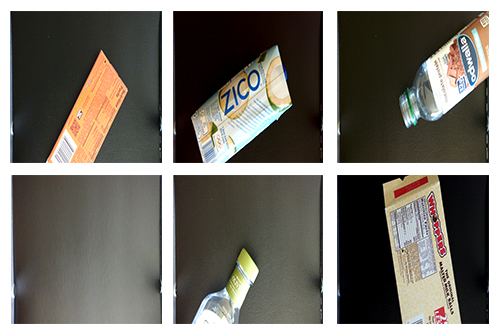
\includegraphics[width=\linewidth]{data-p1-digits}
      \caption{Sample of Supplied Data Set.}
      \label{fig:sample of Supplied Data Set}
\end{figure}

\subsection{Collected Data Set}
The sample data is collected using a USB web cam, each object are taken with different angles, pose, and the size of the image is 256x256, stored in png format. Three Datasets has been collected, they are bottle, can and others.
Because of the limited amount of data, the dataset is augmented by rotating, shifting, shearing the original image to create about 400 images per category. 

\begin{figure}[thpb]
      \centering
      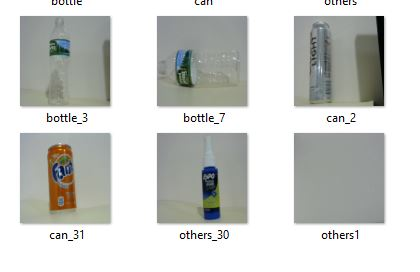
\includegraphics[width=\linewidth]{collected}
      \caption{Sample of collected Data Set.}
      \label{fig:sample of collected Data Set}
\end{figure}

\section{Results}
\subsection{Supplied Data Set}
As Shown in the figure below, the accuracy of the model after training is almost 100\% after 6 epoch.

The accuracy reported by evaluation command is 75.4\%, and the inference time is  around 5ms, which satisfies the requirement to be accurate on or above 75\% with an inference time less than 10ms.

\subsection{Collected Data Set}
As Shown in the figure below, the accuracy of the model on the collected data set after training is almost 100\% after 30 epoch.however the inference time has not been measured.

\begin{figure}[thpb]
      \centering
      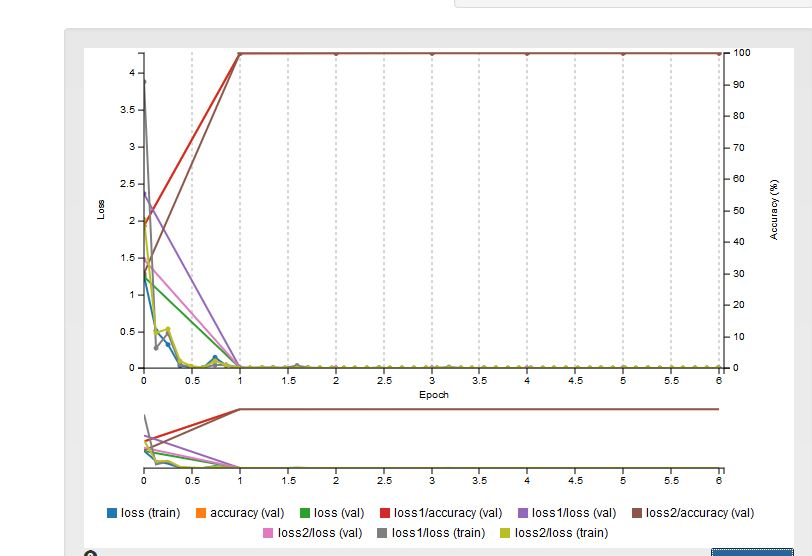
\includegraphics[width=\linewidth]{conveyor}
      \caption{loss and accuracy on supplied data set.}
      \label{fig:loss and accuracy on supplied data set}
      \centering
      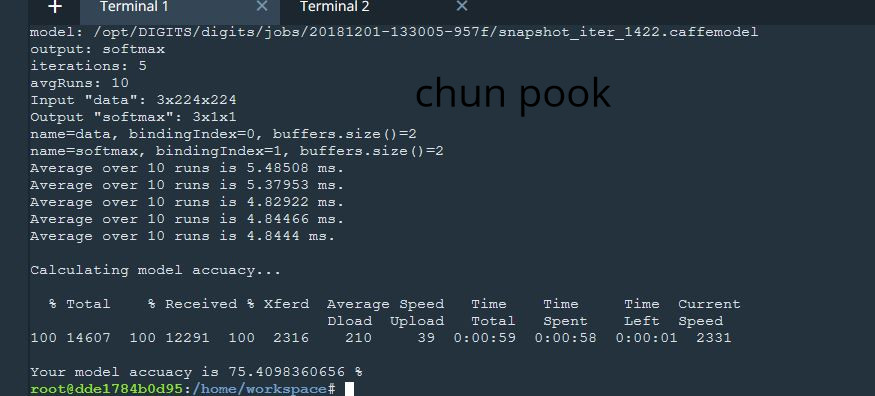
\includegraphics[width=\linewidth]{conveyorevaluate}
      \caption{evaluation on supplied data set.}
      \label{fig:evaluation on supplied data set}
      \centering
      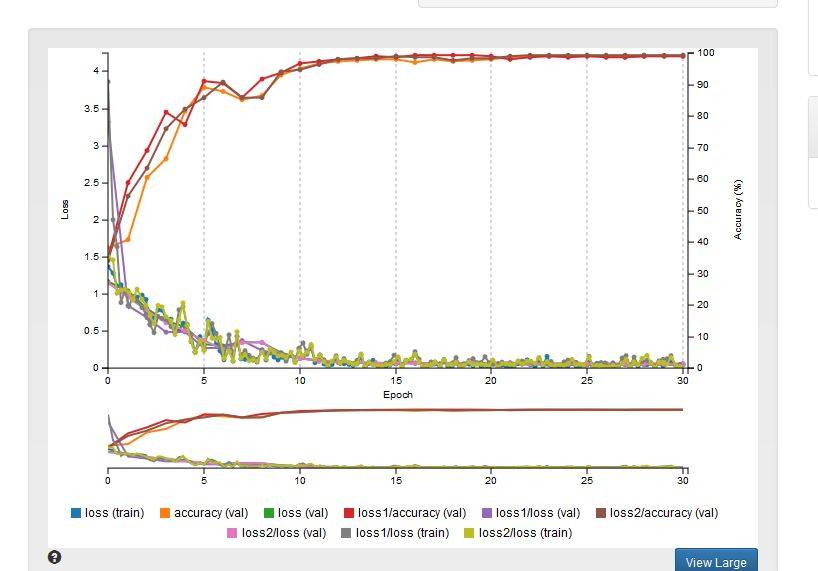
\includegraphics[width=\linewidth]{recycle}
      \caption{loss and accuracy on collected data set.}
      \label{fig:loss and accuracy on collected data set}
\end{figure}

\section{Discussion}
\subsection{supplied Data set}
The model is able to achieve an inference time of around 5ms and accuracy 75.4\% satisfying the requirement. However the accuracy for both training and valuation accuracy is around 100\%. It may be the model is not able to generalize well. Including more variety of images from different source should help alleviate the problem.

\section{Collected Data Set}
The accuracy on the collected data set seems to be too good, achieving almost 100\%. But probably the performance will drop for unseen photos like deformed plastic bottle or can Or bottle with liquid inside.

\section{Conclusion / Future work}
Prototypes for object classification for objects on conveyor belt, and classifier for recycle object has been built.
Further improvements will be to include more object types such as paper, glass etc in the classification process. Also inference time is important to real time application, an improvement will be to make sure the resulting model satisfy real time constraint, e.g. the inference time has to be less than 10ms.
In Real life, bottles or cans are usually slightly deformed, sometimes still have liquid inside, images should include those kind of images to deal with real life situation. 
\end{document}